    \subsection*{Neural Network Perspectives: Classification and Regression}
    
        In this class, we \textbf{won't} focus on the brain analogy, though it did inspire the model.
        
        Instead, we will mostly think of \textbf{neural networks} in terms of what they're able to do, and how they work.
        
        One problem we have struggled with is certain tasks that can't be handled by \textbf{linear} models. We have used \textbf{feature representations} to work on this problem.
        
        Simply, some problems are outside our \textbf{hypothesis} space. But, there's another way: this is where \textbf{neural networks} come in.
        
        By combining lots of simple \textbf{units} ("neurons"), we can get a very \textbf{complex} model for solving our problems.
        
        With such a \textbf{rich} hypothesis class, combined with the power of \textbf{gradient descent}, we can create a model that can do \textbf{classification} or \textbf{regression} for very difficult problems!
            \note{Reminder: "richness" or "expressiveness" of a hypothesis reflect how wide our options are. Neural networks give us many possibilities for models. With more options, we can handle more problems!}\\
            
        \begin{concept}
            \vocab{Neural Networks} can create a very \vocab{rich hypothesis class} by combining many simple \gren{units}.
            
            With this \gren{hypothesis class}, we can handle \purp{regression} or \purp{classification} for very challenging \gren{problems}.
        \end{concept}
    
    \subsection*{Building up a basic neural network}
        
        Let's make sense of what we said above, and \textbf{visualize} what a neural network might look like.
        
        We start with one function: a \textbf{neuron}. This function could be, for example, one we've used before: our logistic \textbf{classifier}, or linear \textbf{regression}. We'll ignore the details for now.
       
        \begin{figure}[H]
            \centering
            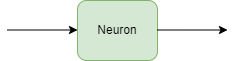
\includegraphics[width=60mm,scale=0.4]{images/nn_images/neuron.png}
        \end{figure}
       
        One neuron might not be very powerful, or \textbf{expressive}. It's useful, but limited. We've seen its weaknesses.
       
        We could try to use \textbf{feature transformations} to help us. But, let's think in a more \textbf{general} way: a transformation is just another \textbf{function} we apply to our input!
       
        \begin{figure}[H]
            \centering
            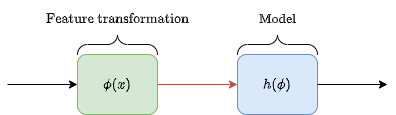
\includegraphics[width=80mm,scale=0.4]{images/nn_images/feature_transform.png}
        \end{figure}
       
        This gives us an \textbf{idea}: rather than trying to think of a single, more \textbf{complex} model, we could \textbf{combine} multiple simple models!
            \note{Note that feature transformations are a bit complex for what we'd usually put in a neuron. But, it gives us the right inspiration.}
       
        \begin{figure}[H]
        \centering
            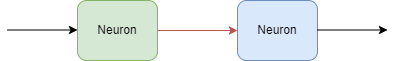
\includegraphics[width=80mm,scale=0.4]{images/nn_images/two_neurons.png}
        \end{figure}
        
        We could repeatedly add more neurons in \textbf{series}: each one being the input to another. And we'll do that later!
        
        But, there's another type of \textbf{complexity} we haven't explored: we could have two neurons in \textbf{parallel}.
            \note{This parallel/series vocabulary is borrowed from circuits. We'll just use it for demonstration: you don't need to remember it.}
        
        \begin{figure}[H]
        \centering
            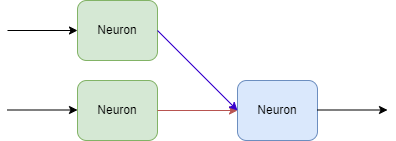
\includegraphics[width=100mm,scale=0.4]{images/nn_images/three_neurons.png}
        \end{figure}
        
        Now, we have \textbf{two} neurons feeding into one output neuron! This already looks like a more \textbf{complicated} model. 
        
        We can go even further: what if we have two outputs as well?
        
        \begin{figure}[H]
        \centering
            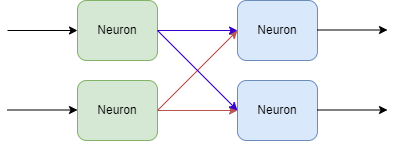
\includegraphics[width=100mm,scale=0.4]{images/nn_images/four_neurons.png}
        \end{figure}
        
        Because we had two \textbf{inputs}, we had to add two new \textbf{links} when we added the output neuron. This is getting difficult to \textbf{view}!
        
        We'll stop here for now, but you can imagine repeatedly \textbf{adding} more neurons in \textbf{parallel} (with the same inputs/outputs) or in \textbf{series} (as an input or output).
        
        And we each addition, the function gets more and more \textbf{complex}: you can create a \textbf{richer} hypothesis class!
        
        We'll explore how to do this \textbf{systematically} later in the chapter.
            \note{By "systematic", we just mean "in a way that's consistent and makes sense".}\\
        
        \begin{definition}
            \vocab{Neural Networks} are a \purp{class} of models that can be used to solve \gren{classification}, \gren{regression}, or other interesting problems.
            
            They create very \purp{rich} hypothesis classes by combining many \gren{simple} models, called \vocab{neurons}, into a \gren{complex} model.
            
            We do this combination \purp{systematically}, so that it is easy to \gren{analyze} and work with our \purp{model}.
            
            This creates a very \purp{flexible} hypothesis, which can be \gren{broken down} into its \purp{simple} parts and what \gren{connects} them.
        \end{definition}